\documentclass[12pt]{article}
\usepackage{amsfonts,amsmath,amssymb,amsthm}
\usepackage{xcolor,enumerate,autobreak}
\usepackage{tikz}
\usetikzlibrary{decorations.markings}
\usetikzlibrary{arrows}

\begin{document}

  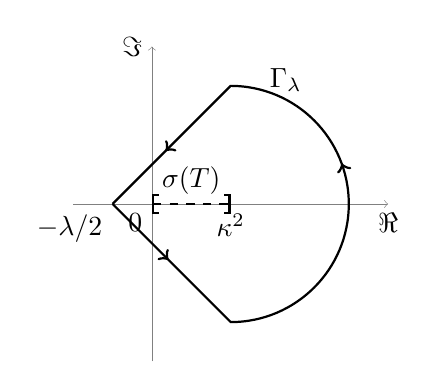
\begin{tikzpicture}
[decoration={markings,
mark=at position 1cm with {\arrow[line width=1pt]{>}},
mark=at position 5cm with {\arrow[line width=1pt]{>}},
mark=at position 8cm with {\arrow[line width=1pt]{>}}
}
]
% The axes
  \draw[help lines,->] (-1,0) -- (3,0) coordinate (xaxis);
  \draw[help lines,->] (0,-2) -- (0,2) coordinate (yaxis);

% The path
%  arc (-90:90:1.5)  -- (0,0.5);
  \path[draw,line width=0.8pt,postaction=decorate] (-0.5,0) node[below left] {$-\lambda/2$} -- (1,-1.5)
  arc (-90:90:1.5)  -- (-0.5,0);
  \draw[{[-]}, line width=0.8pt, dashed] (0,0) -- (1,0) node[below] {$\kappa^2$};

% The labels
  \node[above] at (0.5,0) {$\sigma(T)$};
  \node[below] at (xaxis) {$\Re$};
  \node[left] at (yaxis) {$\Im$};
  \node[below left] {$0$};
  \node[above] at (1.7,1.3) {$\Gamma_\lambda$};
\end{tikzpicture}

\end{document}